\documentclass[12pt]{article}
\usepackage{color}
\usepackage{graphicx}
\usepackage{booktabs}
\usepackage{amsmath}
\usepackage[utf8]{inputenc}
%\usepackage[german]{babel}
\usepackage{multirow}
\usepackage{siunitx}
\usepackage{pbox}
%\usepackage{tabularx}
\usepackage{multirow}
\usepackage{float}
\usepackage{amssymb,amsmath}
\makeatletter
\def\maketag@@@#1{\hbox{\m@th\normalfont\normalsize#1}}
\makeatother
\setlength{\parindent}{0pt}

%\addtolength{\textwidth}{1in}
%\addtolength{\textheight}{1in}
%\addtolength{\evensidemargin}{0.5in}
%\addtolength{\oddsidemargin}{-0.5in}
%\addtolength{\topmargin}{-0.6in}
%\addtolength{\bottommargin}{0.4in}


\usepackage[top = 2.50cm, bottom = 2.50cm, left = 2.75cm, right = 2.50cm]{geometry}

\renewcommand{\floatpagefraction}{1.0}


\begin{document}
\title{PHY118/119 \\ {\bf Hydrostatik/-dynamik}}
\author{Assistent: Simon Flury \\E-mail: simon.flury@uzh.ch\\ }
\maketitle

\section{Wichtig!!!}
Dieses Dokument ist kein offizielles Dokument, es ist weder von Prof.Kilminster noch vom Hauptassistenten abgesegnet, somit kann sich nicht darauf bezogen werden und es wird auch keine Haftung für Fehler übernommen. Es dient einzig und allein als Lernunterstützung von mir an euch und bezieht sich ausschliesslich auf meine Übungsstunde.

\section{Einführung}

\textbf{Aggregatszustände}

\begin{itemize}
\item fest $\rightarrow$Elastizitätslehre
\item flüssig $\rightarrow$ Hydrostatik/-dynamik
\item gasförmig $\rightarrow $Hydrostatik/- dynmaik
\end{itemize}

 Wie wir sehen befasst sich die die Hydrostatik/-dynmaik mit der mit der Beschreibung des Verhaltens von Gasen und Flüssigkeiten. Gase und Flüssigkeiten werden im Innern gleich betrachtet, sprich man betrachtet eine Ansammlung von Teilchen und beschreibt ihre Bewegung als Mittelwert. Der wichtigste Unterschied zwischen diesen beiden Aggregatszuständen ist, dass die Dichte variert:
 \begin{itemize}
 \item flüssig: $\rho = const$ inkompressibel
 \item gasförmig: $\rho(p)$ kompressibel
 \end{itemize}
 \clearpage
 
 \textbf{Definition: Druck}
 In der Statik gilt $v=0$ und somit für die Viskosität $\eta = 0$. Dies impliziert, dass es keine innere Reibung gibt, sprich keine Schubspannung ($\tau = 0$). Zur erinnerung die Schubspannung $\tau = \dfrac{dF_{||}}{dA} $ wobei die Kraft parallel zur Fläche wirkt. Da dies wie gesagt $0$ ist, kann die Kraftrichtung im Fluid nur senkrecht zur Fläche stehen, was der Normalkraft entspricht. Dies bedeutet, dass wir den Spannungszustand im Fluid mit einer einzigen skalaren Grösse, dem Druck, beschreiben können:
 \begin{equation}
 p = \dfrac{F}{A}
 \end{equation}
 Diese Grösse ist ein Skalar, dass heisst sie ist unabhängig von der Richtung (Pascal'sches Prinzip)\\
 \\
 Der Druck wird in der Einheit Pascal $Pa = N/m^2$ angegeben, zudem gebrächlich sind: $1bar = 10^5Pa = 1atm$ und $1Torr = 1mm Hg$
 
 \subsection{Druck in einem Kraftfeld}
 Wir betrachten nun wie sich der Druck in einem externen Kraftfeld (in unserem Fall dem Gravitationsfeld der Erde) verhält.

\begin{figure}[H]
  \centering{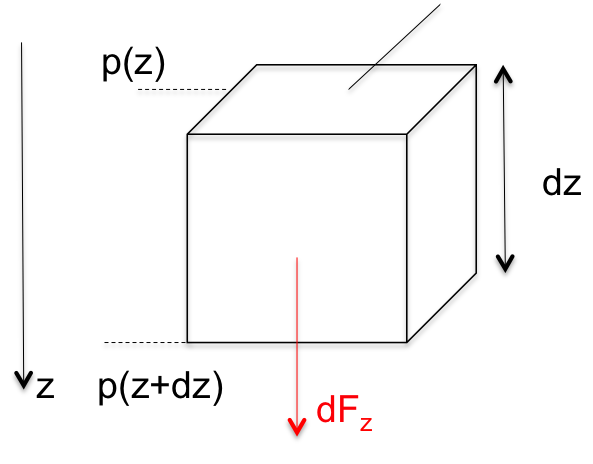
\includegraphics[width=0.2\textwidth]{Hydro1.png}}
  \label{fig:1teil}
\end{figure} 

\begin{equation}
dF_z = \left(p(z+dz)-p(z) \right) dA
\end{equation}
\begin{equation}
f_z = \dfrac{dF_z}{dV} = \dfrac{\left(p(z+dz)-p(z) \right)}{dA \cdot dz} \cdot dA
\end{equation}
\begin{equation}
\rightarrow f_z = \dfrac{dp}{dz}
\end{equation}
Wenn wir nun wie gesagt als Kraftfeld, dass Gravitationfeld der Erde annehmen, erhalten wir:
\begin{equation}
\rho(z) \cdot g = \dfrac{dp}{dt}
\end{equation}

\section{Flüssigkeiten}
 Wir wollen nun eine einfache Situation betrachten, in der wir ein mit einer Flüssigkeit gefülltes Gefäss haben und den Druck in verschiedenen Tiefen bestimmen wollen.
 
 \begin{figure}[H]
  \centering{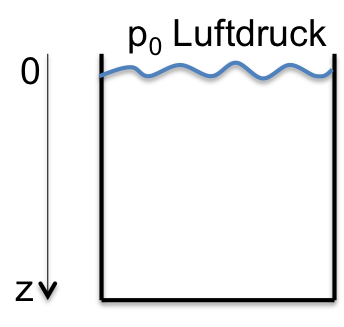
\includegraphics[width=0.2\textwidth]{Hydro2.png}}
  \label{fig:1teil}
\end{figure} 

\begin{equation}
\dfrac{dp}{dz} = \rho \cdot g \quad \mathrm{mit} \quad p(0) = p_0
\end{equation}
Achtung: wir beschreiben eine Flüssigkeit, dass bedeutet die Dichte $\rho$ ist konstant.
\begin{equation}
\rightarrow \quad p(z) = p_0 + \rho \cdot g \cdot z
\end{equation}
für Wasser ($\rho = 1000kg/m^3$) erhalten wir für einen Tiefenunterschied von $10m$ einen Druckunterschied von $1bar = 10^5Pa$

\subsection{Kommunizierende Gefässe}
Wir betrachten ein U-Rohr, welches mit zwei Flüssigeiten gefüllt ist. Unser Interesse gilt dem Höhenverhältnissen der Flüssigkeitssäulen im Rohr.

 \begin{figure}[H]
  \centering{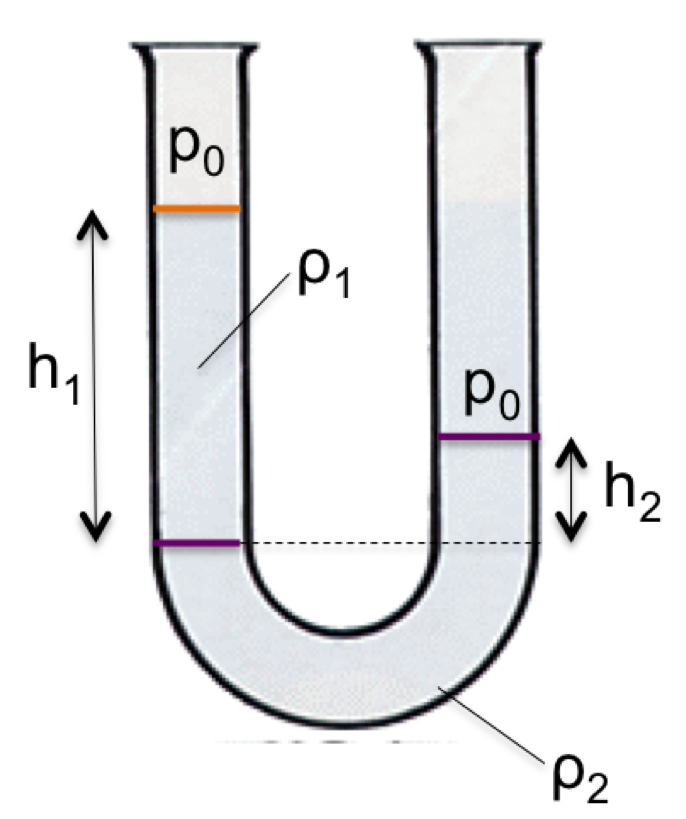
\includegraphics[width=0.2\textwidth]{Hydro3.png}}
  \label{fig:1teil}
\end{figure}
Es ist klar dass auf beiden Seiten der gleiche Druck herschen muss, da sich sich sonst kein Gleichgewicht eintsellt.
\begin{equation}
p_0 + \rho_1 h_1 g = p_0 + \rho_2 h_2 g
\end{equation}
\begin{equation}
\rightarrow \dfrac{\rho_1}{\rho_2} = \dfrac{h_2}{h_1}
\end{equation}

Wir bemerken also, dass die Höhendifferenz nur aufgrund der unterschiedlichen Dichten resultiert und wir aus dieser somit direkt auf das Dichteverhältnis schliessen können.

\subsection{Torricelli}
Hierbei geht es um das berühmte Beispiel eines mit einer Flüssigkeit gefüllten Gefässes, welches auf einer bestimmten Höhe einen Ausfluss hat. Von interesse ist hierbei vorallem die Fliesgeschwindigkeit.
 \begin{figure}[H]
  \centering{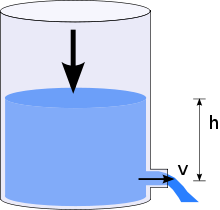
\includegraphics[width=0.2\textwidth]{Hydro4.png}}
  \label{fig:1teil}
\end{figure}

\begin{equation}
dF = \left(p(h)-p_0 \right) \cdot dA \quad \rightarrow \quad dW = \left(p(h)-p_0 \right) \cdot dA \cdot dx
\end{equation}

\begin{equation}
dW  = \dfrac{1}{2} \cdot dm \cdot v^2 = \dfrac{1}{2} \rho \cdot dV \cdot v^2 = \dfrac{1}{2} \rho \cdot v^2 \cdot dA \cdot dx
\end{equation}

\begin{equation}
p(h)-p_0 = \dfrac{1}{2} \rho \cdot v^2 \quad \Leftrightarrow \quad p_0 + \rho \cdot g \cdot h -p_0 = \dfrac{1}{2} \rho \cdot v^2
\end{equation}
somit erhalten wir für die Fliessgeschwindigkeit:
\begin{equation}
v = \sqrt{2gh}
\end{equation}

\section{Gase}
Was wir nun versuchen wollen ist einen Ausdruck für den Druck in Gasen (z.B. Atmosphäre), in Abhängigkeit der Höhe z zu finden, dies wird uns direkt auf die \textbf{barometrische Höhenformel} führen.\\
\\
Bei Gasen ist die Dichte abhängig vom Druck, somit gilt  die Gleichung  $\dfrac{dp}{dz} = -\rho (p) \cdot g$. Mit diesem Ausdruck können wir noch nicht viel anfangen, da wir nicht wissen, wie die Dichte vom Druck abhängt. Wir nehmen uns desahlb die \textbf{Ideale Gasgleichung} $p \cdot V = \nu \cdot R \cdot T$ zur hilfe. Für ein Mol gilt: $m = m_{mol}$ und $\nu = 1$. Damit können wir die folgende Umformung machen:
\begin{equation}
V = \dfrac{RT}{p} \quad \rightarrow \quad \rho = \dfrac{m_{mol} \cdot p}{RT}
\end{equation}
Dies führt uns nun auf folgende Differentialgleichung (ihr müsst nicht verstehen wie man die löst):
\begin{equation}
\dfrac{dp}{dz} = - \dfrac{m_{mol}}{RT} \cdot g \cdot p \qquad \mathrm{mit} \qquad p(0) = p_0 = (1013hPa)
\end{equation}
deren Lösung die \textbf{barometrische Höhenformel} ergibt
\begin{equation}
p(z) = p_0 \cdot \exp \left(- \dfrac{m_{mol}g}{RT} \cdot z \right)
\end{equation}
\clearpage

\section{Auftrieb}
Wenn wir ein Objekt in einem Fluid haben, welches sich zudem noch in einem Kraftfeld z.B. Gravitationsfeld befindet, wirkt auf dieses Objekt die sogennate Auftriebskraft. Sie ist äquivalent zur Gewichtskraft des vom Objekt verdrängten Fluids und resultiert aus Druckunterschieden entlang des Körpers.
 \begin{figure}[H]
  \centering{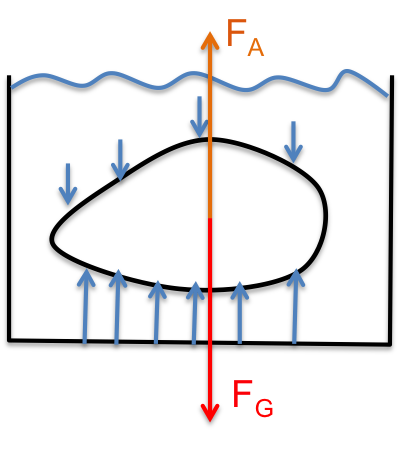
\includegraphics[width=0.2\textwidth]{Hydro6.png}}
  \label{fig:1teil}
\end{figure}
Der Druck nimmt mit zunehmender Tiefe zu, somit stellt sich einen Druckdifferenz bezüglich der Ober- und Unterseite des Objektes ein, welcher zu eine Kraft $F_A$ der sogenanten Auftriebskraft führt, welche der Gravitationskraft $F_G$ entgegengesetzt ist.
Betrachten wir das Kräftegleichgewicht ergibt sich folgendes:
\begin{equation}
\vec{F_A} + \vec{F_G} = 0 \quad \rightarrow \quad \vec{F_A} = -\vec{F_G} = -m\vec{g} = - \int_V \rho_{fl} \cdot \vec{g} \cdot dV
\end{equation}
Also erhalten wir für den Betrag der Auftriebskraft:
\begin{equation}
F_A = \int_V \rho_{fl} \cdot g \cdot dV = V_{verdrängt} \cdot \rho_{fl} \cdot g
\end{equation}
wobei über das vom Objekt verdrängte Volumen integriert wird.
Somit erhalten wir als resultierende Kraft:
\begin{equation}
F = F_G - F_A = \int_V (\rho_{K} - \rho_{fl}) \cdot g \cdot dV
\end{equation}
Durch das Einführen der Grösse: $\bar{\rho} = \dfrac{\int_V \rho dV}{\int_V dV}$ ist es uns möglich die Folgenden Aussagen zu tätigen:
\begin{itemize}
\item $\bar{\rho_K} > \bar{\rho_{fl}} \rightarrow$ Kraft in Richtung des Gravitationsfeldes $\rightarrow$ sinkt.
\item $\bar{\rho_K} < \bar{\rho_{fl}} \rightarrow$ Kraft entgegen des Gravitationsfeldes $\rightarrow$ steigt.
\end{itemize}
\clearpage
\section{Hydrodynmaik}
Um die Dynamik eines Systems konsistent zu beschreiben benötigt man Elemente aus der Vektoralgebra. Ich versuche dies wenn möglich zu vermeiden, da es nicht Teil eures Lenstoffes ist. Es kann sein das mir dies nicht überall gelingt, dann betrachtet es einfach als Zusatzinfo, welche ihr aber keines Falls an der Prüfung können müsst.
\\
\\
Im dynamischen Fall $\vec{v} \ne 0$ beschreiben wir die Situation mittels Strömungen.
 \begin{figure}[H]
  \centering{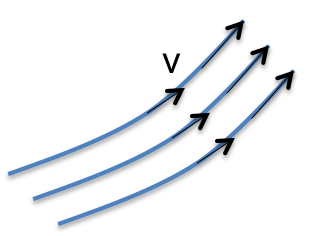
\includegraphics[width=0.2\textwidth]{Hydro7.png}}
  \label{fig:1teil}
\end{figure}
Diese Linen sind die sogennaten Strömungslinien. Diese stellen das Verhalten der Strömung graphisch dar. Was wir eigentlich hier sehen ist ein Vektorfeld $\vec{v}(\vec{r},t)$.\\
Wir wollen den Fall von \textbf{stationären Strömungen} betrachten.\\
\\
Für eine stationäre Situtation gilt $\dfrac{\partial \vec{v}}{\partial t} = 0$, dies bedeutet jedoch nicht das $\dfrac{d\vec{ v}}{dt} = 0$, denn
\begin{equation}
\dfrac{d\vec{v}}{dt} = \dfrac{\partial \vec{v}}{\partial x} \cdot \dfrac{dx}{dt} + \dfrac{\partial \vec{v}}{\partial y} \cdot \dfrac{dy}{dt} + \dfrac{\partial \vec{v}}{\partial z} \cdot \dfrac{dz}{dt} + \dfrac{\partial \vec{v}}{\partial t}
\end{equation}
Der Unterschied ist, dass sich bei $\dfrac{d\vec{v}}{dt} = 0$ weder die Geometrie eures Systems mit der Zeit ändern darf, noch die Flussgeschwindigkeit, bzw. Flussrichtung.$\dfrac{\partial \vec{v}}{\partial t} = 0$ sagt nur, dass sich bei gegebener Geomtrie nicht auf einmal die Fliessgeschwindigkeit oder Fliessrichtung ändern darf.
\\
\\
In der Hydrodynmaik sind zwei Dinge von zentraler Bedeutung:
\begin{itemize}
\item Massenerhaltung $\rightarrow$ Kontinuitätsgleichung
\item Energieerhaltung $\rightarrow$ Bernoulligleichung
\end{itemize}
\textbf{Kontinuitätsgleichung}
\\
Wir wenden uns zuerst der Massenerhaltung zu, welche wir am Beispiel folgender Situation erläutern wollen.

 \begin{figure}[H]
  \centering{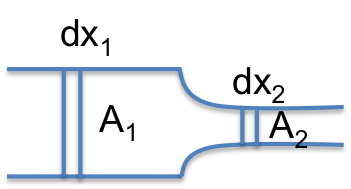
\includegraphics[width=0.3\textwidth]{Hydro8.png}}
  \label{fig:1teil}
\end{figure}
Nun betrachten wir wieder zwei infinitesimale Massenelemente. Wegen der Massenerhaltung müssen sie an Stelle 1 und 2 gleich sein
\begin{equation}
dm_1 = dm_2 \quad \rightarrow \quad \rho_1 \cdot dV_1 = \rho_2 \cdot dV_2 \quad \rightarrow \quad \rho_1 \cdot A_1 \cdot dx_1 = \rho_2 \cdot A_2 \cdot dx_2
\end{equation}
leiten wir nun beide Seiten nach der Zeit ab, erhalten wir:
\begin{equation}
\rho_1 \cdot A_1 \cdot v_1 = \rho_2 \cdot A_2 \cdot v_2
\end{equation}
Wir betrachten hier Flüssigkeiten, welche inkompressibel sind, somit ist $\rho_1 = \rho_2$ was uns auf die bekannte Kontiniutätsgleichung führt:
\begin{equation}
A_1 \cdot v_1 = A_2 \cdot v_2
\end{equation}
\\
\\ 
Eine kleine Anmerkung: Wenn ihr nach dem Begriff Kontinuitätsgleichung sucht, werdet ihr folgende Formel finden $\dfrac{\partial \rho}{\partial t} + div(\vec{j}) = 0$ dies bedeutet, dass die Änderung der Massenstromdichte gleich der zeitlichen Dichteänderung ist. Diese Gleichung ist die allgemeine Kontinuitätsgleichung in 3dim, für den spezialfall eines Rohrsystems und in 1dim, ergibt sich unsere hergeleitete Gleichung.
\\
\\\textbf{Bernoulligleichung}
\\
Wir wollen ein Massenelement eines strömenden Fluids unter den Aspekten Arbeit, kinetische und potentielle Energie, betrachten
 \begin{figure}[H]
  \centering{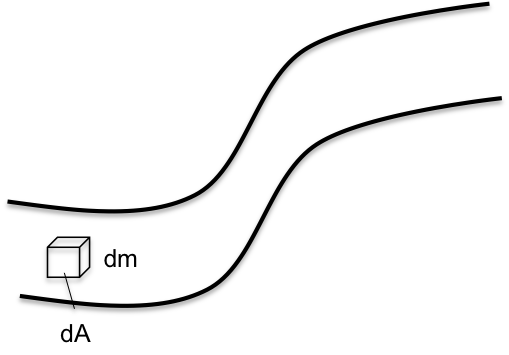
\includegraphics[width=0.3\textwidth]{Hydro9.png}}
  \label{fig:1teil}
\end{figure}
Reibung wird vernachlässigt, sprich $\eta = 0$.
\begin{equation}
dW = dF \cdot dx = p \cdot dA \cdot dx = p \cdot dV
\end{equation}
\begin{equation}
dT = \dfrac{1}{2} dm \cdot v^2 = \dfrac{1}{2} \rho \cdot v^2 \cdot dV
\end{equation}
\begin{equation}
dU = dm \cdot h \cdot g = \rho \cdot h \cdot g \cdot dV
\end{equation}
daraus ergibt sich die Bernoulligleichung
\begin{equation}
\left(p + \dfrac{1}{2} \rho \cdot v^2 + \rho \cdot g \cdot h \right) = p_0 = const
\end{equation}
dabei sind die Terme der reihe nach: hydrostatisch, dynamisch, Schweredruck
\end{document}
